
\section{Design of the internet}

\begin{definition}
    {The internet}

    \begin{itemize}
        \item Global system of computer networks that use the TCP/IP protocol suite to link devices worldwide.
        \item Network of networks
    \end{itemize}
\end{definition}

\begin{knBox}
    {IP addresses}

    IP addresses are generally organized by organization.
\end{knBox}

\subsection{Sending data}

\begin{definition}
    {Circuit switching}

    Single stream of information per path. To handle multiple input streams, we need to multiplex:

    \begin{itemize}
        \item \textbf{Frequency Division: } Optical / electromagnetic waves divided into narrow frequency bands
        \item \textbf{Time Division: } Time slots are assigned to each communication channel
    \end{itemize}

    \textit{Pros:}
    \begin{itemize}
        \item \textbf{Guaranteed performance}: Dedicated resources for each input stream
        \item \textbf{Fast transfers}: Resources are reserved ahead of time
    \end{itemize}
    \textit{Cons:}
    \begin{itemize}
        \item \textbf{Wasted bandwidth if traffic is bursty}: Reserved resources may go unused during idle periods
        \item \textbf{Setup time}: Takes time to setup dedicated path and resources
        \item \textbf{Poor fault tolerance}: If part of the reserved path fails, the system may not recover easily
    \end{itemize}
\end{definition}

\begin{definition}
    {Packet switching}

    Each "packet" of data is self-contained, with header and payload. Each packet is independently routed to the destination.

    Overall allows more conversations and better utilization of resources.
\end{definition}

\subsection{Protocols}

\begin{definition}
    {Protocol}
    A set of rules governing the exchange or transmission of data between devices. It defines:
    \begin{itemize}
        \item Roles of communicating entities
        \item Format / order of messages
        \item Actions taken on event
    \end{itemize}
    Fully-defined protocol must provide a proper action for any event in any state
\end{definition}

\begin{theorem}
    {Request-Response Protocols}
    A class of protocols where a client sends a request and waits for a response from the server.

    Some rules might get \textbf{complicated} when considering slow responses, large sizes, etc.
\end{theorem}

\begin{knBox}
    {Linked Finite State Machines}

    A protocol can be modeled as a set of linked finite state machines (FSMs), one for each role in the protocol.
\end{knBox}

\begin{definition}
    {Protocol Stack}

    \begin{tabular}{|l|l|l|}
        \hline
        \textbf{Layer} & \textbf{Functionality}                                          & \textbf{Example} \\
        \hline
        Application    & Proper formatting by recipient                                  & HTTP, FTP        \\
        \hline
        Transport      & Identify processes on machine, ordering and recovering          & TCP, UDP         \\
        \hline
        Network        & Routes data through routers to destination machine, ports       & IP address       \\
        \hline
        Link           & Routes data between adjacent devices through direct connections & Ethernet         \\
        \hline
        Physical       & Encodes data properly for physical medium                       & BASE xx          \\
        \hline
    \end{tabular}
\end{definition}

\begin{theorem}
    {Sending data through the stack}

    As the internet has many routers, the path is not as simple as a direct connection between client and server:

    \begin{center}
        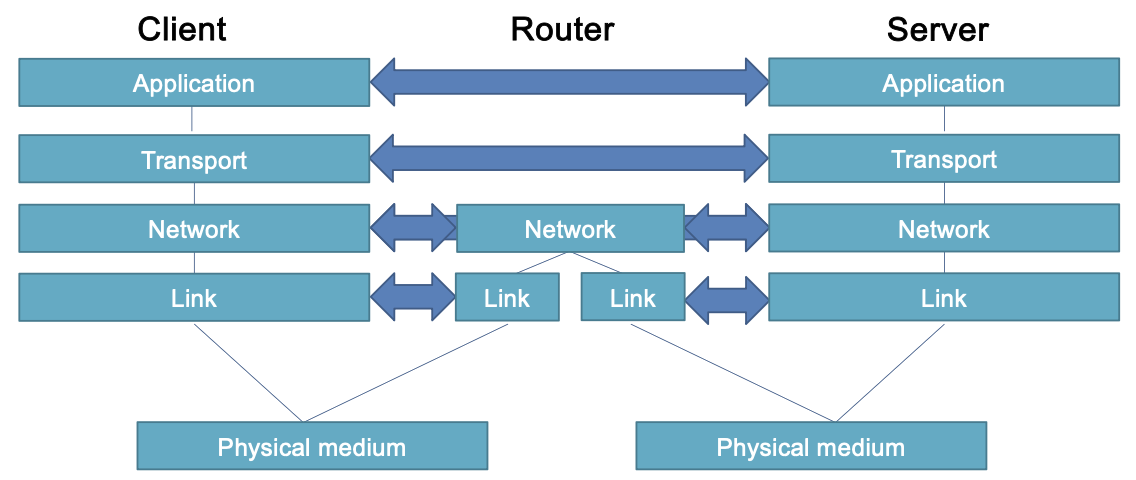
\includegraphics[width=0.7\textwidth]{./images/m01-l02-1.png}
    \end{center}
\end{theorem}

\begin{theorem}
    {Protocol layering and data}

    From the stack, each layer takes data from the above layer, adds header information to create a new data unit, and passes it to the layer below.

    \begin{center}
        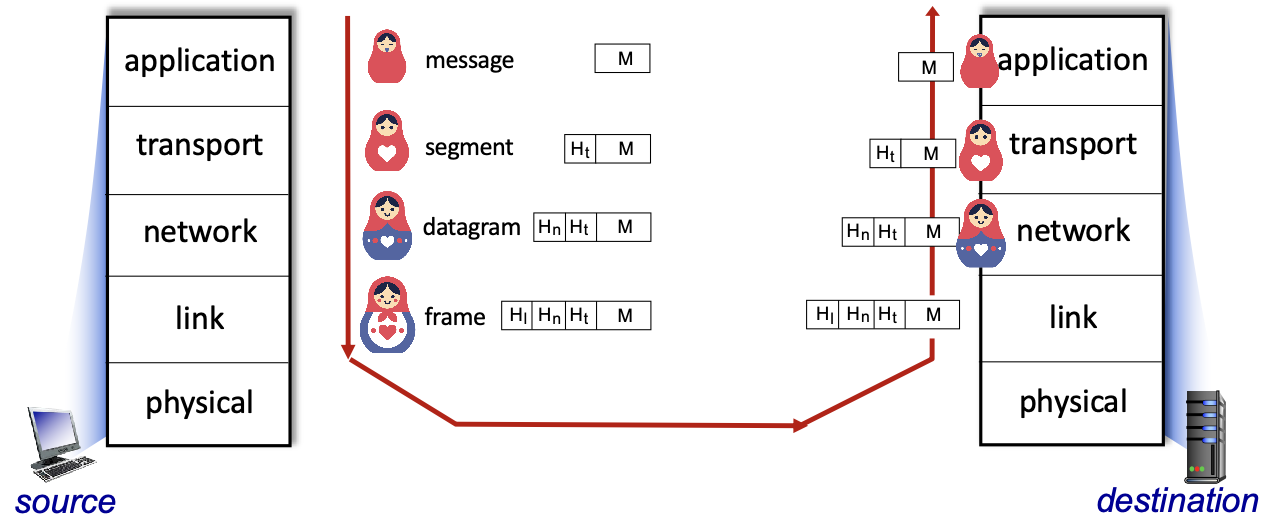
\includegraphics[width=0.45\textwidth]{./images/m01-l02-2.png}
        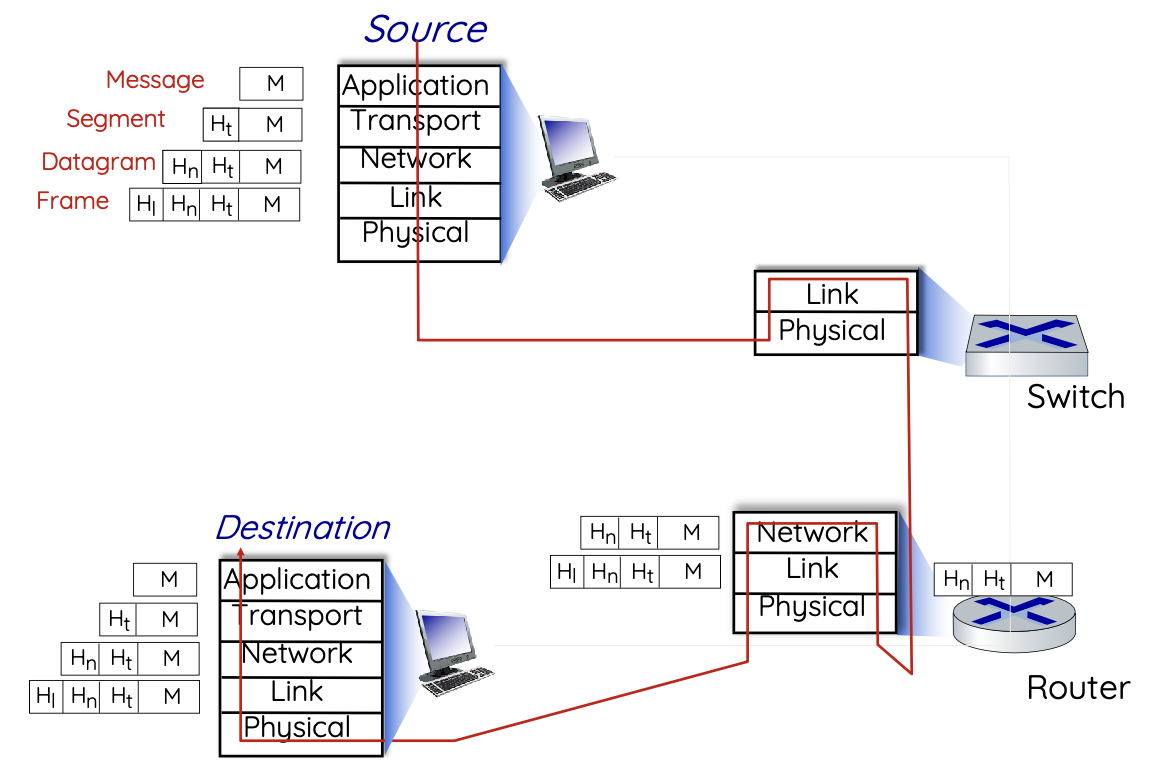
\includegraphics[width=0.45\textwidth]{./images/m01-l02-3.png}
    \end{center}
\end{theorem}